\chapter{Présentation du sujet}
Ayant intégré une équipe travaillant sur un projet existant, je n'ai pas réalisé
un travail de mon côté mais plutôt ajouté de nouvelles fonctionnalités à ce
projet. C'est pourquoi ce chapitre reprend les différentes fonctionnalités que
j'ai développées après une petite introduction du projet global.

\section{Elaastic}
Elaastic est un outil pour concevoir et diffuser des contenus pédagogiques. Il
permet de concevoir des supports pédagogiques structurés, interactifs et
indépendants du format de destination. Il offre la possibilité de diffuser ces
supports sous forme de diaporama ou sous forme de publication au format livre ou
au format site interactif vers un \gloss{ent} par exemple.

\begin{figure}[h]
  \centering
  \includegraphics[scale=0.35]{images/elaastic_blue.pdf}%
  \caption{Logo d'Elaastic}
  \label{fig:elaastic}
\end{figure}

Les cours créés avec Elaastic sont organisés en arbre sur trois niveaux :
\begin{itemize}
  \item Section
	\begin{itemize}
	  \item Sous-section
		\begin{itemize}
		  \item Unité
		\end{itemize}
	\end{itemize}
\end{itemize}

Des ressources comme des images ou des documents externes peuvent être ajoutés à
ces cours pour les enrichir. Nous verrons également qu'il est maintenant
possible d'ajouter des questions interactives en tant qu'unité de cour.\\

D'un point de vue technique, Elaastic se découpe en deux parties. Une partie
Grails pour le corps et la partie \gloss{back-end}. Le système de persistance
des données est assurée par Mongo pour la version de développement. La version
déployée en production s'appuie sur une base de données Postgre SQL. Côté
\gloss{front-end}, l'interface utilisateur est conçu grâce à AngularJS, un
framework Javascript. Cette structure est illustrée par la figure
\ref{fig:webapp} page \pageref{fig:webapp}.

\begin{figure}[h]
  \centering
  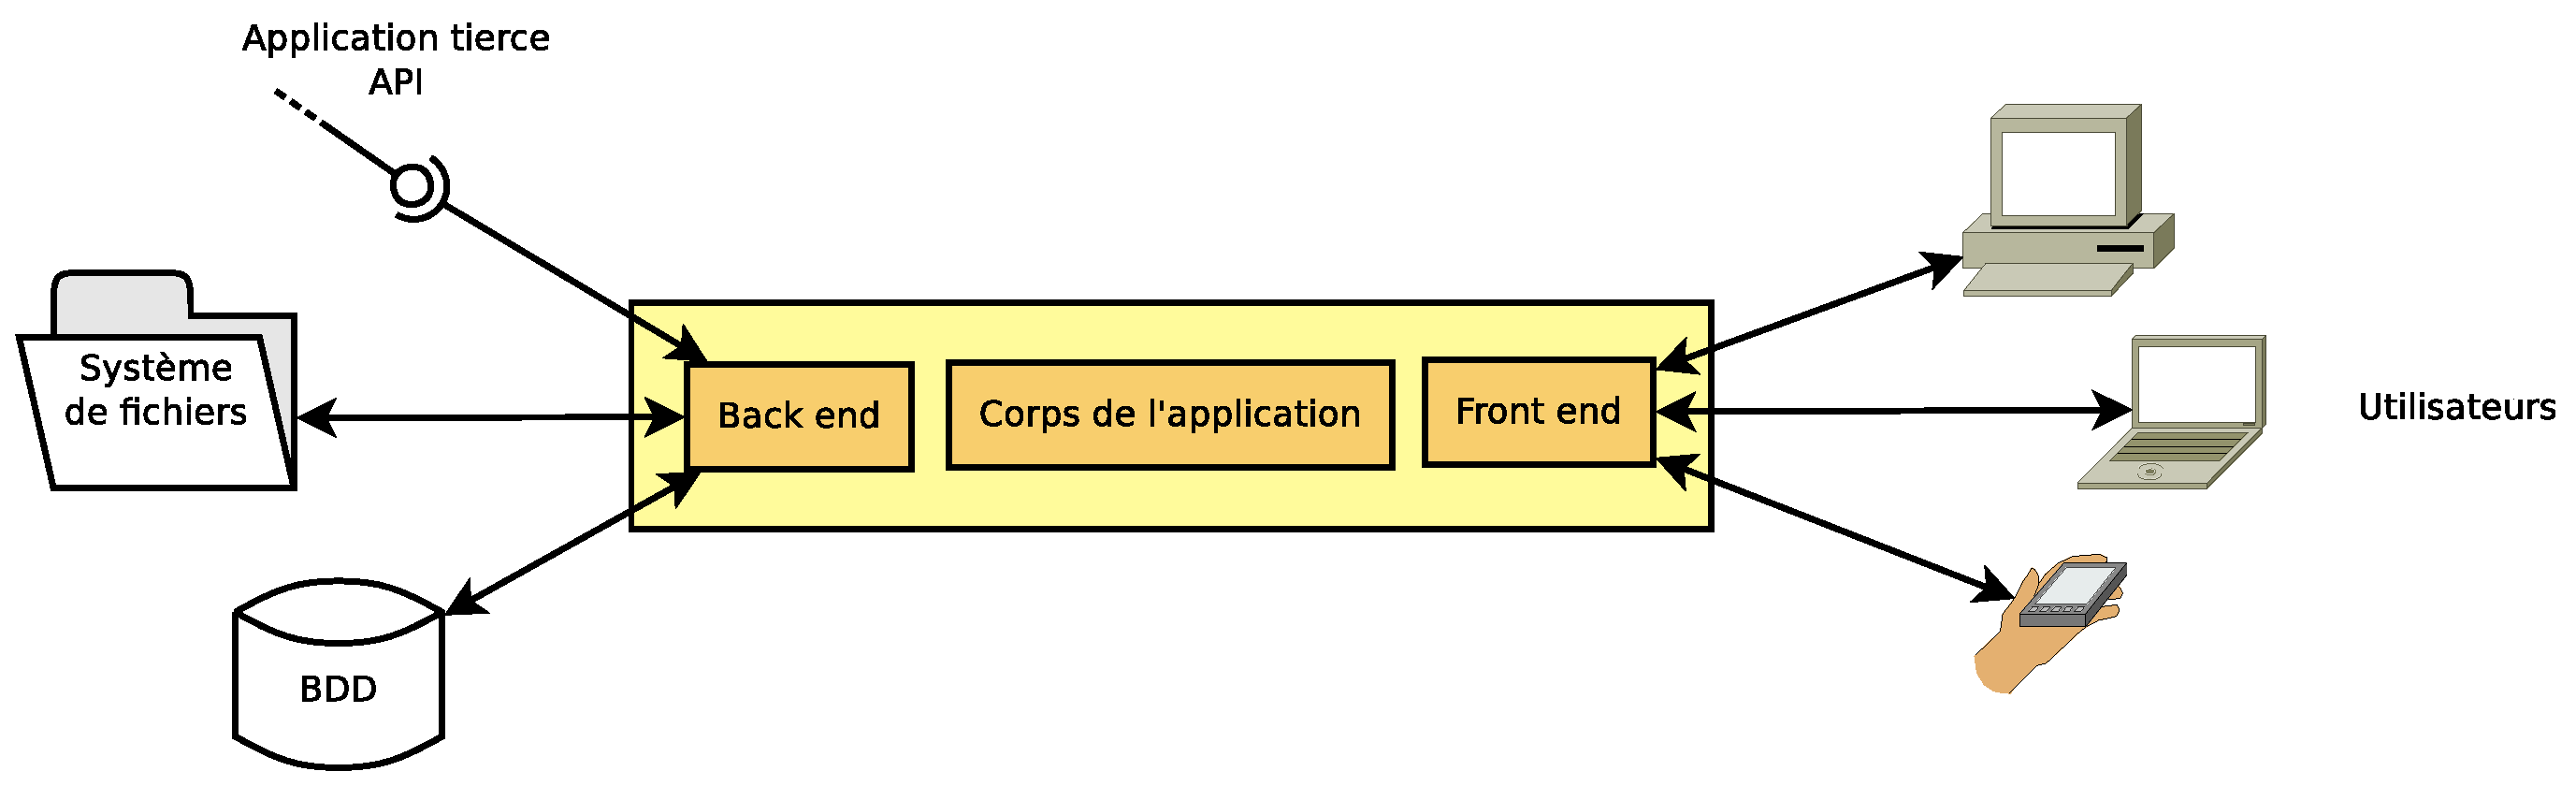
\includegraphics[scale=0.3]{images/webapp.eps}%
  \caption{Illustration du \og front end \fg{} et du \og back end \fg{} par
rapport au corps de l'application.}
  \label{fig:webapp}
\end{figure}

Pour ma part, j'ai essentiellement travaillé sur le corps et la partie back end.
Les sections qui suivent détaillent les fonctionnalités sur lesquelles j'ai
travaillé.

\subsection{Paquetage de Contenu IMS}
\Gloss{imscp} est un format standard d'échange d'information structurées
en arbre -- chapitre, section, sous-section par exemple -- défini par l'IMS
GLC\footnote{IMS Global Learning Consortium}. Cette structure correspond aux
cours créés avec Elaastic et s'adapte bien en format d'exportation. Une des
motivations à fournir ce format d'exportation était que c'est un format
compris par Moodle, plateforme utilisée par Franck et John dans leur activité
d'enseignement. Une fois le paquetage généré, il peut être directement importé
dans Moodle.

Mon travail sur cette fonctionnalité a été d'intégrer au système d'export déjà
existant la possibilité d'exporter un cours créé avec Elaastic au format
\gloss{imscp}.

\subsection{WebDAV}
\Gloss{webdav} est un protocole d'échange et d'édition collaborative de fichier.
Là encore, la motivation était l'intégration à d'autres \gloss{lms} comme
Moodle. En effet, Moodle peut être configuré pour se connecter à des
serveurs \gloss{webdav} pour récupérer ou déposer des fichiers.

L'objectif de cette fonctionnalité était de permettre à l'utilisateur de
configurer un serveur \gloss{webdav} afin de pouvoir déposer des cours dans les
différents formats d'exportation disponibles.

\subsection{Artifact}
Un problème qui est apparu avec la complexification des exportations est le
temps que met l'application à générer ces documents. Un système de cache a été
imaginé pour ne pas avoir à réexporter des cours qui n'auraient pas été modifiés
entre deux exportations. Ces cours générés une première fois dans un format donné
correspondent à un artéfact ({\em artifact} en anglais).

Mon travail sur les artéfacts a été de définir leur structure pour la
persistance des données et de mettre en place un système de cache afin de ne
pas utiliser du temps processeur inutilement et fournir un service plus rapide
quand cela est possible.

\subsection{Diffusion}
Un des objectifs d'Elaastic est de pouvoir diffuser des cours dans plusieurs
formats afin que d'autres personnes -- notamment les étudiants -- puissent y
accéder en dehors des cours. C'est pourquoi il a fallu définir ce qu'était une
diffusion d'un point de vue technique et comment l'intégrer à l'application. Une
première version simple d'une diffusion permet d'accéder à un cours dans
une version donnée dans les formats d'exportation disponibles.

Mon travail sur ce point a été de créer une page contenant une diffusion pour un
cours particulier regroupant les différents formats dans lesquels le cours est
disponible.

\subsection{Question interactive}
Franck a travaillé sur Tsaap-Notes, un outil de micro-blogging pour la prise de
note collaborative durant les cours magistraux. Cet outil permet de créer des
notes dans un format de questions interactives auxquelles les étudiants
répondent en temps réel durant les cours.

Dans une optique de couplage de ce système de prise de note collaborative avec
les cours créés depuis Elaastic, il faudrait que l'utilisateur puissent créer des
unités de cours dans ce format de question interactive.

Mon travail là-dessus a été de rendre possible la saisie par
l'utilisateur d'une unité de cours spéciale qui sera une question interactive.
Les questions seront rédigées au format Moodle GIFT puis analysées et converties
pour l'intégration dans les formats d'exportations.

\section{Démarche méthodologique}
\label{methodo}
Pour chaque activité réalisée, plusieurs marqueurs de suivi de projet étaient à
faire suivre et à mettre à jour au fur et à mesure de l'avancement des tâches.

Pour la gestion de projet et du code source nous utilisions Jira et Git de
manières très couplées. Jira nous permet de découper et d'organiser le travail à
faire et les anomalies détectées. Ainsi nous avions des {\em stories}, des tâche
et sous-tâches, ou des bogues. Jira attribue à chaque élément un identifiant unique
de la forme EL-XXX\footnote{EL étant l'abréviation du projet et XXX un numéro
unique}.

Là où le couplage avec Git intervient, c'est au niveau du nommage des branches.
Nous organisions chaque branche de développement en fonction de l'élément Jira
auquel elle faisait référence. Ainsi, chaque branche correspondait à une et une
seule \og fiche Jira \fg{}. De plus, nous gardions cet identifiant dans les
messages de commits pour permettre leur suivi une fois intégré dans la branche
principale.\\

Une fois le développement de la fonctionnalité terminée, les tests correspondants
écrits et validés et le code nettoyé, la branche passait en {\em \og to review
\fg{} } sur notre tableau Kanban. Une nouvelle branche Git était alors créée
avec l'historique des commits nettoyé. Cette branche reprenait le nom de la
précédente et contenait en plus le marqueur \og ready \fg{}.

Une fois le code revu par John, il me faisait des retours sur ce qu'il avait pu
noter. J'apportais ensuite les modifications retenues et je mettais à jour la
branche Git correspondante pour l'intégration à la branche principale de
développement.\\

De manière plus globale mais toujours dans la méthodologie de travail, nous
faisions des \og daily meeting \fg{} avec John et Vincent afin de tenir compte du
travail fait la journée passée et de ce sur quoi nous allions travailler pour la
journée à venir.\\

Un dernier point sur la démarche de travail que je vais aborder ici est la phase
de test. Pour chaque fonctionnalité développée, une contrainte de validation
était l'écriture de tests pour une couverture de code optimale. Pour vérifier
cette couverture de code, nous utilisions le plugin de couverture de code
fournit avec IntelliJ IDEA.

Pour l'écriture des tests -- ou plus précisément des spécifications -- nous
avons utilisé le framework Spock. C'est un framework pour écrire des tests sous
forme de spécifications. Il permet de spécifier le comportement de chaque méthode d'une
classe dans la classe de test -- spécification -- correspondante. Ce framework permet de faire
des tests sur le comportement de la classe testée en simulant ses interactions
avec de faux objets, des \gloss{mock}. Pour faire cela, il nous permet de suivre
le principe du \og given, when, then \fg{}. Ce principe consiste à spécifier un
état de base -- given -- à lui appliquer un stimulus, un appel de fonction sur un
objet réel par exemple -- when -- et à vérifier que les différentes
interactions fonctionnent et que l'objet réel a bien changé d'état -- then.


